
We research two main cases:
\begin{enumerate}
\item  The fairness among two Reno-Connections with different link latencys
\item The fairness among two Cubic-Connections with different link latencys
\end{enumerate}
The following parameters are constant in our model. The \textit{OnOffApplication} sends with a Rate of $R=5Mbps$. The packet size of the \textit{OnOffApplication} is $Packet size = 1024$. The bottleneck link $b$ has a bandwith of $R_b = 2Mbps$ and a latency of $RTT_b = 200ms$. The link latency $L1$ is the variable in our simulation and has values between $(5ms, 10ms, 20ms, 50ms)$. All data rates in the table are averages over the five simulation runs. Each of the five repetitions runs is seeded with a different error rate $p_{err} = (0.000001, 0.000002, 0.000003, 0.000004, 0.000005)$. This simulation should run without queues in the router $R$.

\subsubsection*{1. Case: Fairness among two Reno-Connections}


\begin{table}[H]
\centering
\begin{tabular}{|l|l|l|l|}
\hline
\textbf{RTT L1} & \textbf{RTT L2} & \textbf{Average $Rx_A$ in KB/s} & \textbf{Average $Rx_B$ in KB/s} \\ \hline
5ms             & 10ms            &          20.07               &         70.88                \\ \hline
10ms            & 10ms            &         24.53                &           70.56              \\ \hline
20ms            & 10ms            &         23.41                &         72.45                \\ \hline
50ms            & 10ms            &          22.21               &           75.53              \\ \hline
\end{tabular}
\end{table}

\begin{figure}[H]
	\centering
	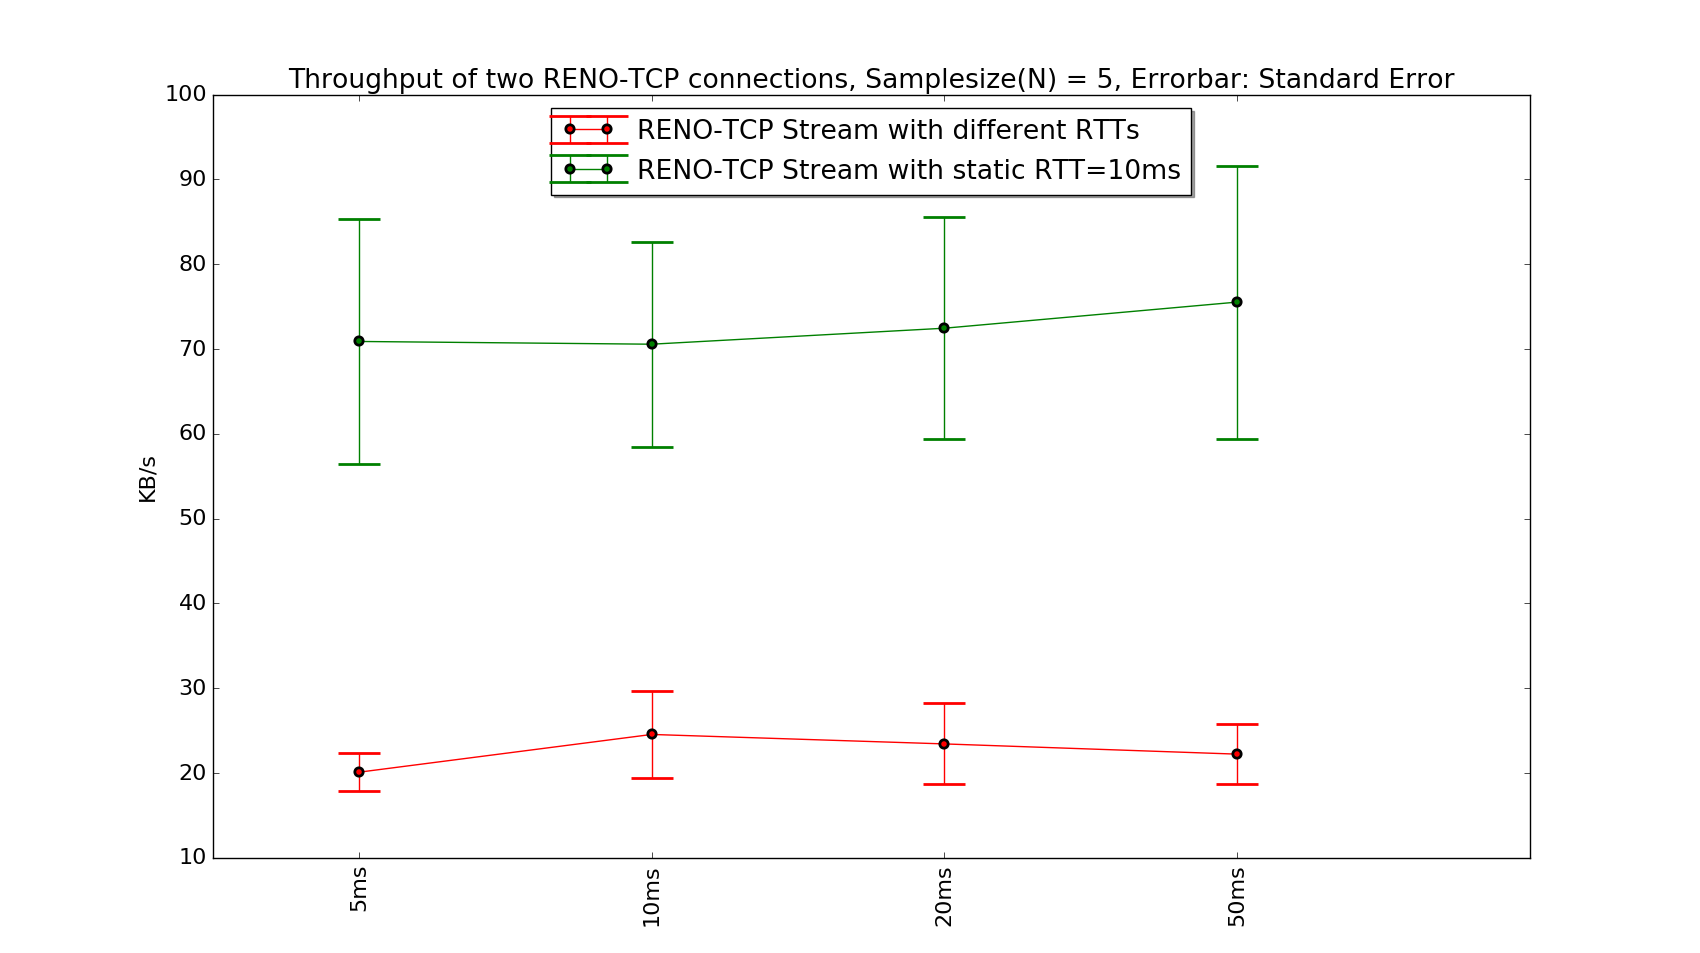
\includegraphics[width=6in]{img/reno.png}
	\caption[reno]
	{Comparision of throughput of two TCP Reno connections.}
\end{figure}

As we can see in the figure 2, the two Reno connections do not converge to a fair usage of the availabe bandwith. Instead, the TCP connection sending from node B over link $L2$ has a significantly higher throughput (around 3 times higher) compared to the TCP connection sending from node A. We would have expected, that the bandwith usage of the two TCP-NewReno connections converges to a fair usage over time. The different RTT's do not explain this strange behavior. However, we can observe that, the higher the RTT for the TCP stream sending from node A, the lower its throughput becomes and the higher the throughput of the other TCP stream becomes. This simulated behavior is predicted by our mathematical model.
\begin{table}[H]
\centering
\begin{tabular}{|l|l|l|l|}
\hline
\textbf{RTT L1} & \textbf{RTT L2} & \textbf{Corrupt Tx A} & \textbf{Corrupt Tx B} \\ \hline
5ms             & 10ms            &        16.0              &         92.4              \\ \hline
10ms            & 10ms            &         22.4              &        83.4               \\ \hline
20ms            & 10ms            &       23.6                &         68.2              \\ \hline
50ms            & 10ms            &       17.8                &         134.8              \\ \hline
\end{tabular}
\end{table}
The number of lost packages of the two TCP streams can be seen in the table above. There is no real insight to derive from the package loss here, other than it indicates that package loss is rather random and consistent. Of course the TCP flow sending from node B has roughly 3 times more package losses than the stream sending from node A, equivalent to their throughputs.

\subsubsection*{2. Case: Fairness among two Cubic-Connections}

\begin{table}[H]
\centering
\begin{tabular}{|l|l|l|l|}
\hline
\textbf{RTT L1} & \textbf{RTT L2} & \textbf{Average $Rx_A$ in KB/s} & \textbf{Average $Rx_B$ in KB/s} \\ \hline
5ms             & 10ms            &          74.08               &         72.26                \\ \hline
10ms            & 10ms            &         72.42                &           67.72              \\ \hline
20ms            & 10ms            &         69.51                &         66.37                \\ \hline
50ms            & 10ms            &          61.94               &           73.34              \\ \hline
\end{tabular}
\end{table}

We can observe in figure 3, that the two cubic connections are very efficient in sharing equal parts of bandwiths over a bottleneck link. In comparasion to the two Reno connection discussed above, the whole bandwith gets efficiently used. When we increase the RTT of one connection (The red plot in figure 3), the throughput of this connections suffers and the throughput of the competing cubic connection (the green plot in figure 3) increases. This behavior however is only starting to become visible with at a $RTT=50ms$. Additonally, we can only hypothesize that the RTT has this influence, since the differences in bandwith at $RTT=50ms$ are not significant. Furthermore, a sample size of N=5 repetitions is much too small to reliable compare two TCP streams. We should have included more simulation runs with even higher RTT's for the red connection. A good pick would have been: $latency=(5ms, 10ms, 20ms, 50ms, 100ms, 250ms, 500ms)$ to reveal bandwith patterns with rising RTT.

\begin{figure}[H]
	\centering
	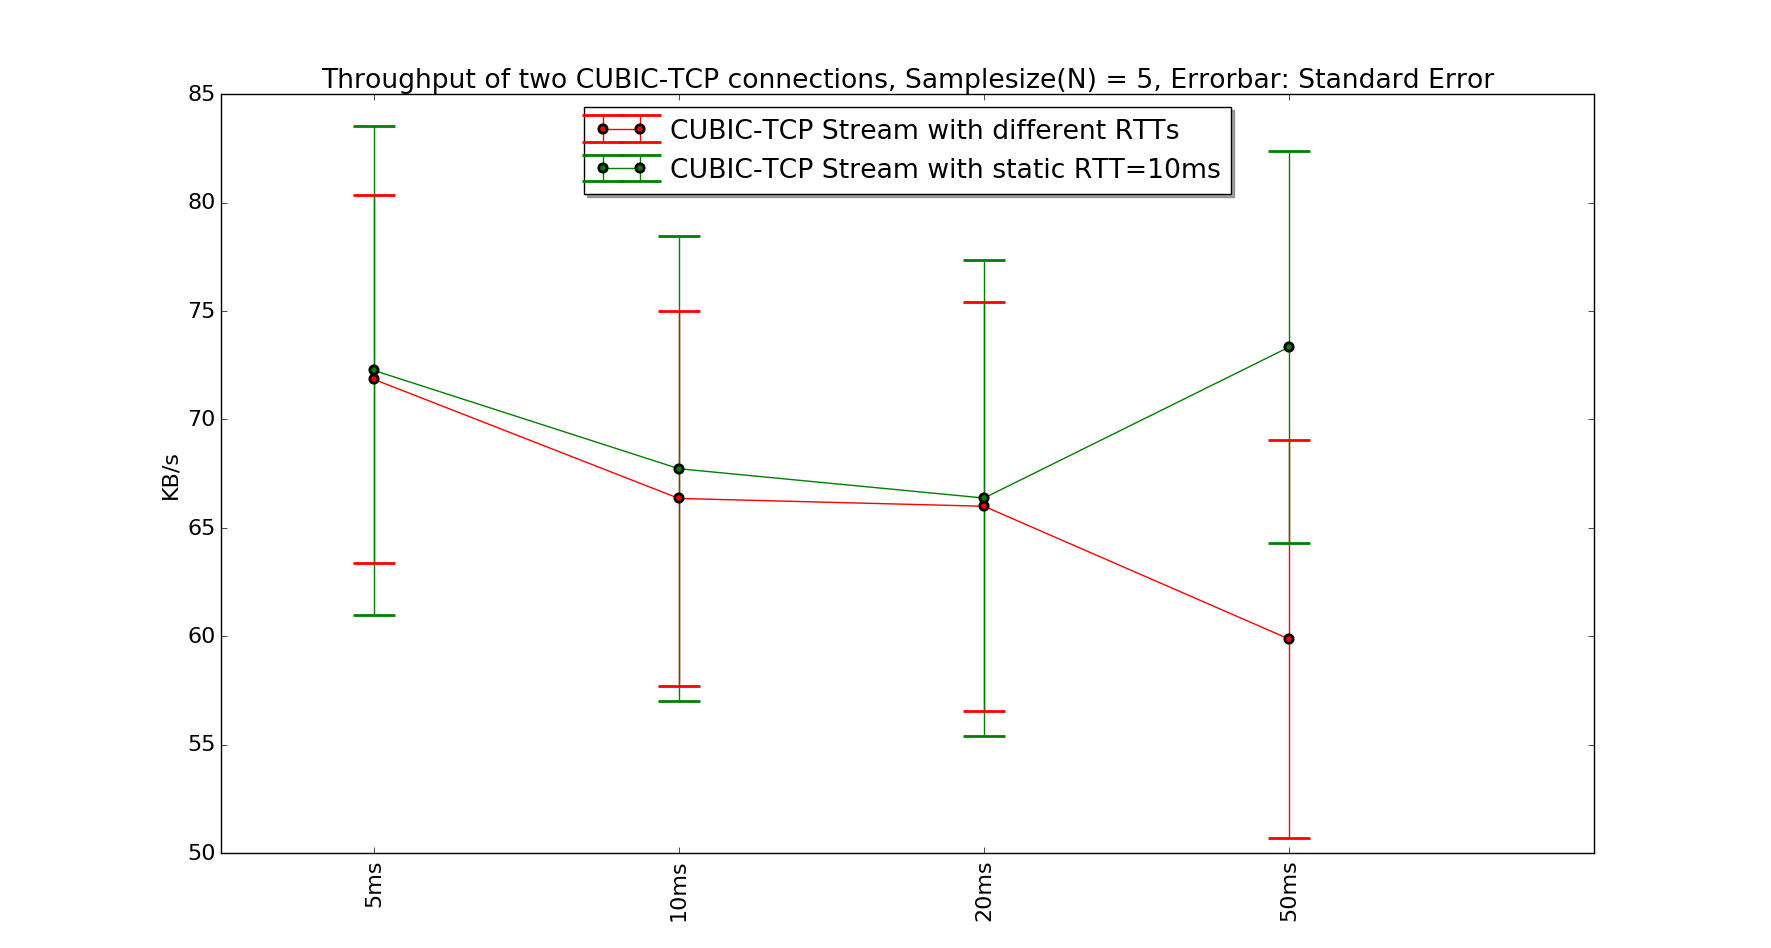
\includegraphics[width=6in]{img/cubic.png}
	\caption[reno]
	\label{fig:cubic}
	{Comparision of throughput of two Cubic connections.}
\end{figure}

The number of lost packages of the two TCP streams can be seen in the table below. As in the case with lost packages in two Reno connections, there is no additional information to be derived, other than package loss occurs on the bottleneck link.
\begin{table}[H]
\centering
\begin{tabular}{|l|l|l|l|}
\hline
\textbf{RTT L1} & \textbf{RTT L2} & \textbf{Corrupt Tx A} & \textbf{Corrupt Tx B} \\ \hline
5ms             & 10ms            &        70.0               &         112.4              \\ \hline
10ms            & 10ms            &         146.2              &        62.4               \\ \hline
20ms            & 10ms            &       85.4                &         132.8              \\ \hline
50ms            & 10ms            &       76.8                &         91.0              \\ \hline
\end{tabular}
\end{table}